\documentclass{standalone}
\usepackage{tikz}
\usepackage{tabularx}
\usepackage{colortbl}
\usepackage{booktabs}

\begin{document}
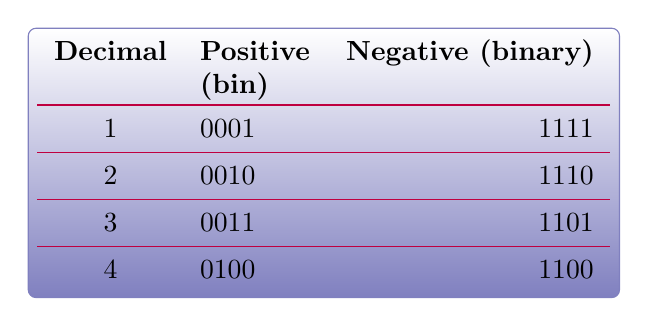
\begin{tikzpicture}[tab_style/.style={
		draw=blue!50!black!50,
		top color=white,
		bottom color=blue!50!black!50,
		rounded corners=1mm
	}]

\node[tab_style](tbl) {
\begin{tabularx}{.6\textwidth}{cXrcc}
\arrayrulecolor{purple}
\textbf{Decimal} & \textbf{Positive (bin)} & \textbf{Negative (binary)} \\
\toprule
1 & 0001 & 1111 \\
\midrule
2 & 0010 & 1110 \\
\midrule
3 & 0011 & 1101 \\
\midrule
4 & 0100 & 1100
\end{tabularx}
};

\end{tikzpicture}
\end{document}
